\documentclass[a4paper]{report}

\usepackage{NielsPackage}

\lstset{language=HTML}

\hypersetup{
	pdfauthor = {Niels Doorn},
	pdftitle = {Javascript Oefeningen},
	pdfsubject = {HTML, CSS, JavaScript},
	pdfkeywords = {HTML,css,lesbrief},
	pdfcreator = {NielsDoorn/RocVanTwente}
}

\rhead{\textsc{Javascript Oefeningen}}
\lhead{}
\chead{}
\lfoot{Niels Doorn \copyright~2012}
\cfoot{}
\rfoot{\thepage}

\fancypagestyle{plain}{
	\fancyhf{}
	\fancyfoot[L]{Niels Doorn, ROC van Twente \copyright~2012}
	\fancyfoot[C]{}
	\fancyfoot[R]{\thepage}
	\renewcommand{\headrulewidth}{0pt}
	\renewcommand{\footrulewidth}{0.4pt}
}

\begin{document}

\chapter*{\textcolor{seccol}{Javascript} Oefeningen}

\section*{Inleiding}
In de vorige lesbrief hebben we kennisgemaakt met JavaScript. Deze lesbrief gaat verder met een aantal oefeningen om JavaScript wat meer onder de knie te krijgen. Deze oefeningen moet je in een les maken en af laten tekenen door je docent!

\section*{Elementen selecteren uit de DOM}
In de vorige lesbrief hebben we al kort kennisgemaakt met het selecteren van elementen uit de DOM. Nu kan dat niet alleen met behulp van het id van een element, maar je kunt ook alle elementen met een bepaalde class opvragen. Dit kan met de functie \textbf{getElementsByClassName}. Deze functie kan meerdere elementen teruggeven in de vorm van een lijst. Hieronder een voorbeeld. 

\lstinputlisting{code/oef1.html}

\clearpage

\lstinputlisting{code/scriptOef1.js}

\noindent \textbf{Opdracht 1.1:} Wat verschijnt er in je console als je deze pagina in je browser opent?
\\
\\
\noindent \textbf{Opdracht 1.2:} Voeg een vierde blokje toe, pas de \emph{JavaScript} code zo aan dat alle blokje met de class blokje, een rode achtergrondkleur krijgen.
\\
\\
\noindent \textbf{Opdracht 1.3:} Selecteer met de JavaScript functie \textbf{getElementById} het derde blokje en geef dit blokje een groene border met een dikte van 4px.

\section*{Het Canvas}
In HTML5 is er een Canvas tag toegevoegd die het mogelijk maakt om te tekenen op een webpagina! Met behulp van JavaScript kunnen we rechte lijnen, curves, rechthoeken, circles, tekst en afbeeldingen toevoegen aan een canvas. Een Canvas kan in 2D en in 3D gebruikt worden. Deze opdrachten maken gebruik van de 2D mogelijkheden. Eerst een voorbeeld van de HTML en de JavaScript om op een canvas te tekenen. Het resultaat van deze code ziet er zo uit:

\begin{center}
\resizebox{40mm}{!}{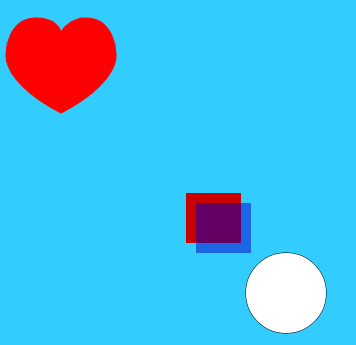
\includegraphics{canvasResult}}
\end{center}

\clearpage

\lstinputlisting{code/oef2.html}


\lstinputlisting{code/scriptOef2.js}


\noindent \textbf{Opdracht 2.1:} Maak een tekening van een smiley op een canvas.
\\
\\
\noindent \textbf{Bonusopdracht 2.2:} Zoek uit hoe je met de \textbf{drawImage} functie een afbeelding op een canvas kunt tekenen.
\\
\\
\noindent De volgende lessen gaan we verder hiermee en gaan we kijken of we iets op het canvas met behulp van het toetsenborde kunnen laten bewegen!

\section*{Handige links}
Moz dev canvas tutorials: \url{http://goo.gl/216I}. 
\\
\noindent Handige canvas cheatsheet: \url{http://goo.gl/8G2ag}.


\end{document}